\part{Calculos Manuales}

\section{Teoria}

Para poder realizar el analisis de la ataguia se debe tener en cuenta los siguientes conceptos:

\subsection{Red de Flujo}

Una red de flujo es un conjunto de tuberias y nodos que se interconectan para transportar un fluido de un punto a otro. En este caso, se busca analizar la red de flujo de agua que se encuentra en la ataguia. Para esto se utilizo como guia el libro \cite{budhu2011}.

\subsection{Caudal de infiltracion}

El caudal de infiltracion es la cantidad de agua que se filtra a traves de un suelo. En este caso, se busca analizar el caudal de infiltracion que se produce en la ataguia.
El cual se calcula con la siguiente formula:

\begin{equation}
    Q = k \cdot \frac{\Delta H}{n_{p}} \cdot n_{s}
\end{equation}

\subsection{Presion de Poros}

La presion de poros es la presion que se ejerce en los poros de un suelo. En este caso, se busca analizar la presion de poros que se produce en la ataguia.

Para esto se utilizaron las siguientes ecuaciones:

\begin{equation}
    H_{t} = H_{0} + \Delta H
\end{equation}

\begin{equation}
    H_{t} = z_{g} + \frac{u_{w}}{\gamma_{w}}
\end{equation}

\begin{equation}
    \Delta H_{i} = \frac{\Delta H}{n_{p}} \cdot n_{i}
\end{equation}

\begin{equation}
    u_{w} = (H_{t} - z_{g}) \cdot \gamma_{w}
\end{equation}

\subsection{Presion neta en la ataguia}

La presion neta en la ataguia es la presion que se ejerce en la ataguia. En este caso, se deben comparar las presiones que se ejercen en cada lado de la ataguia.

\subsection{Gradiente Hidraulico Maximo}

El gradiente hidraulico maximo es la pendiente maxima que puede tener una tuberia para que el agua fluya sin problemas. En este caso, se busca analizar el gradiente hidraulico maximo que se produce en la ataguia.

Para esto se utilizo la siguiente formula:

\begin{equation}
    i_{max} = \frac{\Delta H}{L_{min}}
\end{equation}

\subsection{Gradiente Hidraulico Critico}

El gradiente hidraulico critico es la pendiente minima que puede tener una tuberia para que el agua fluya sin problemas. En este caso, se busca analizar el gradiente hidraulico critico que se produce en la ataguia.7

Para esto se utilizo la siguiente formula:

\begin{equation}
    i_{crit} = \frac{\gamma '}{\gamma_{w}}
\end{equation}


\subsection{Factor de Seguridad}

El factor de seguridad es la relacion entre la resistencia de un material y la carga que se le aplica. En este caso, se busca analizar el factor de seguridad que se produce en la ataguia.

Para esto se utilizo la siguiente formula:

\begin{equation}
    FS = \frac{\gamma_{sat} - \gamma_{w}}{i \cdot \gamma_{w}}
\end{equation}


\section{Resultados}

\subsection{Diagramas Escala 1:200}

\begin{figure}[H]
    \centering
    \begin{minipage}{0.32\textwidth}
        \centering
        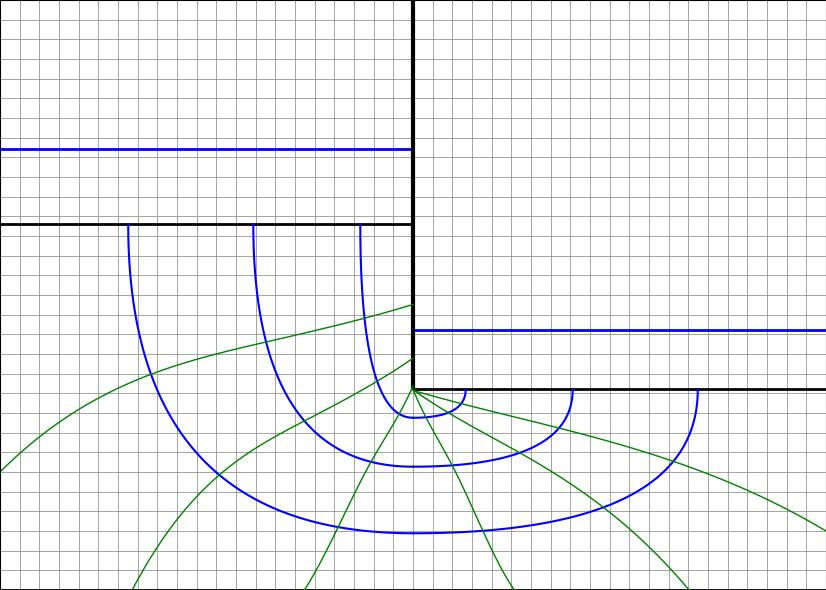
\includegraphics[width=\textwidth]{GRAFICOS/caso_1.jpg}
        \caption{Caso 1}
    \end{minipage}
    \begin{minipage}{0.32\textwidth}
        \centering
        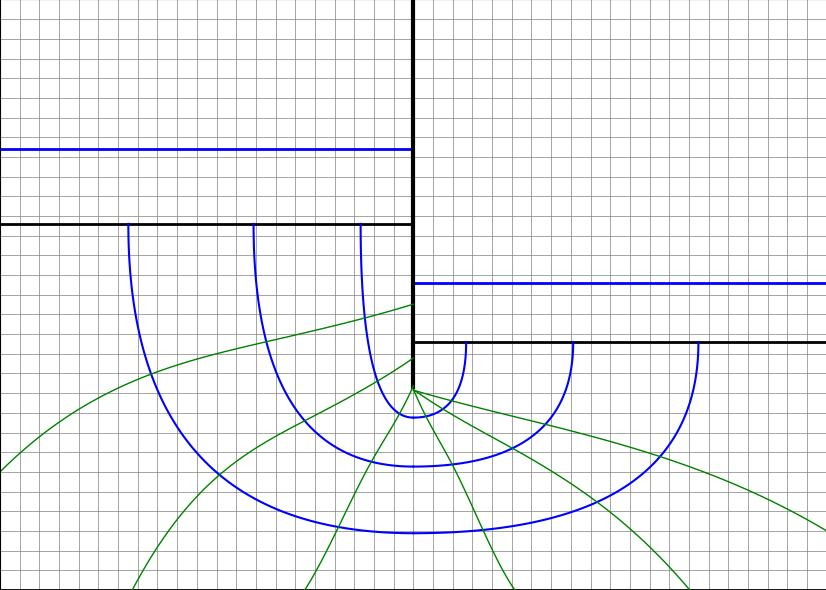
\includegraphics[width=\textwidth]{GRAFICOS/caso_2.jpg}
        \caption{Caso 2}
    \end{minipage}
    \begin{minipage}{0.32\textwidth}
        \centering
        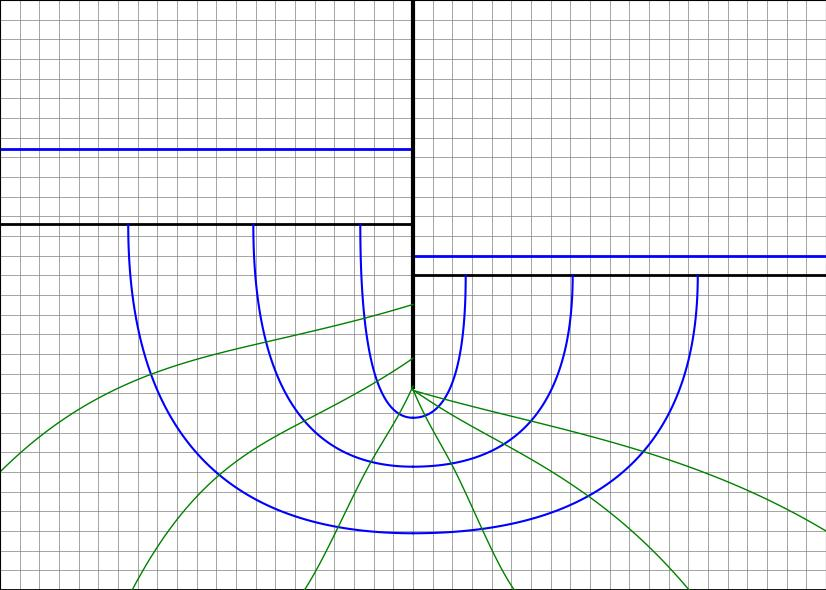
\includegraphics[width=\textwidth]{GRAFICOS/caso_3.jpg}
        \caption{Caso 3}
    \end{minipage}
  \end{figure}

\subsection{Presion de Poros}

\subsubsection{Distribucion Presiones}

\begin{figure}[H]
    \centering
    \begin{minipage}{0.32\textwidth}
        \centering
        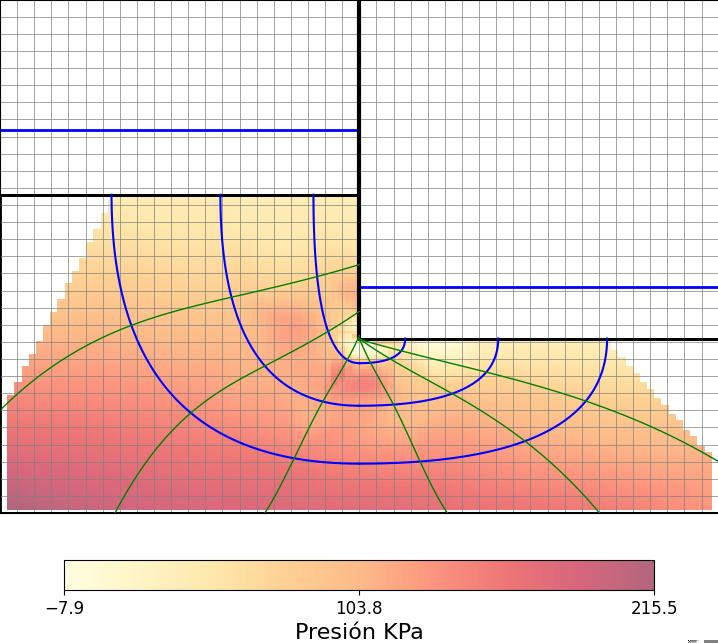
\includegraphics[width=\textwidth]{GRAFICOS/caso_1_presion_poros.jpg}
        \caption{Caso 1 Presion Poros}
    \end{minipage}
    \begin{minipage}{0.32\textwidth}
        \centering
        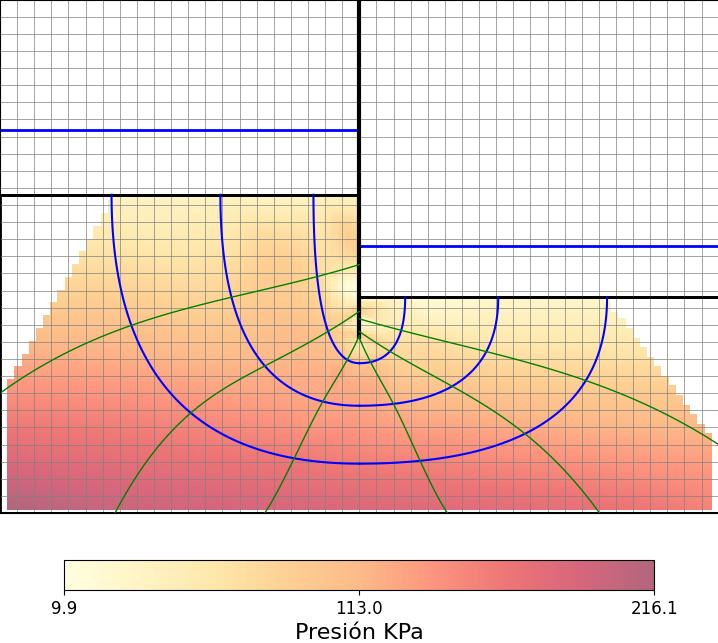
\includegraphics[width=\textwidth]{GRAFICOS/caso_2_presion_poros.jpg}
        \caption{Caso 2 Presion Poros}
    \end{minipage}
    \begin{minipage}{0.32\textwidth}
        \centering
        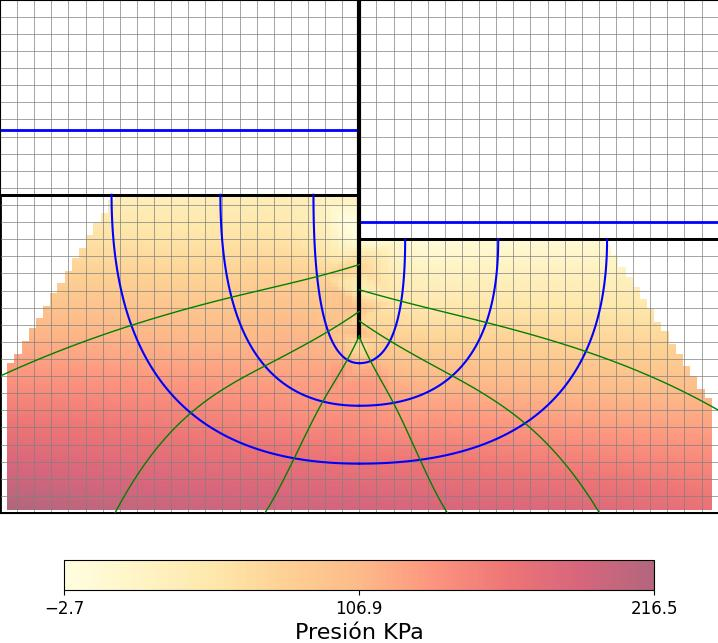
\includegraphics[width=\textwidth]{GRAFICOS/caso_3_presion_poros.jpg}
        \caption{Caso 3 Presion Poros}
    \end{minipage}
\end{figure}

\subsubsection{Presiones Totales}

\begin{figure}[H]
    \centering
    \begin{minipage}{0.32\textwidth}
        \centering
        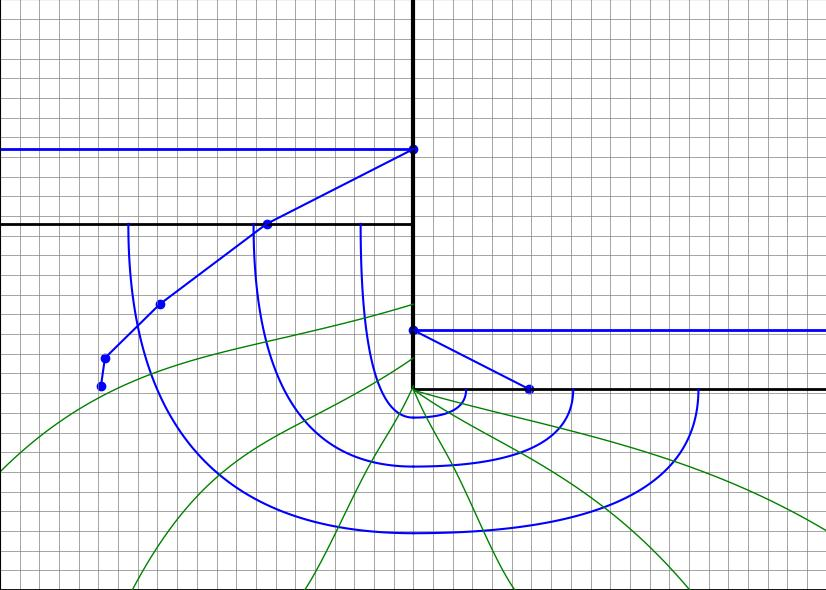
\includegraphics[width=\textwidth]{GRAFICOS/caso_1_presion_ataguia_total.jpg}
        \caption{Caso 1 Presion Ataguia Total}
    \end{minipage}
    \begin{minipage}{0.32\textwidth}
        \centering
        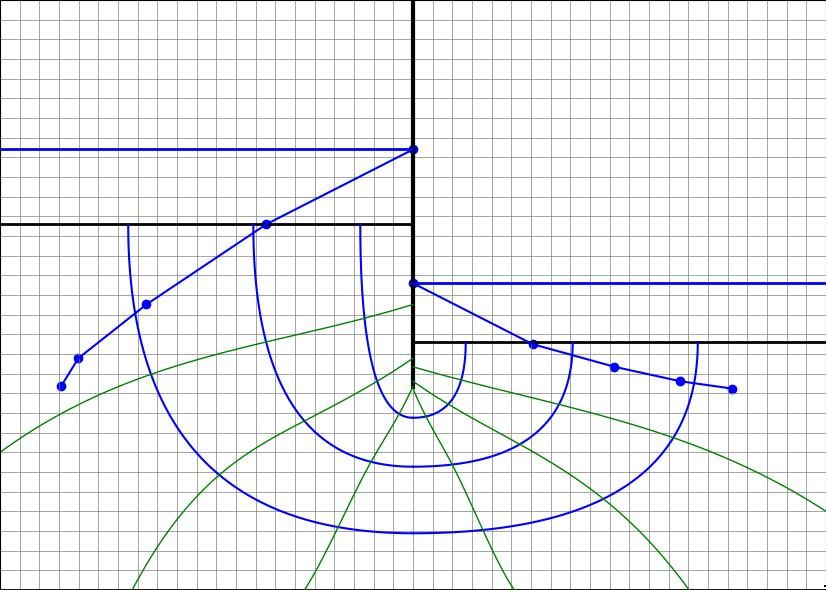
\includegraphics[width=\textwidth]{GRAFICOS/caso_2_presion_ataguia_total.jpg}
        \caption{Caso 2 Presion Ataguia Total}
    \end{minipage}
    \begin{minipage}{0.32\textwidth}
        \centering
        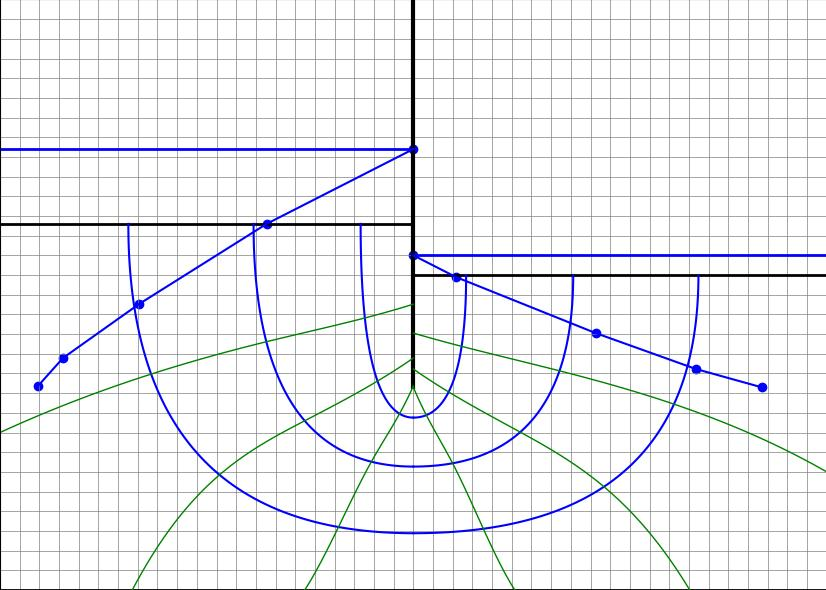
\includegraphics[width=\textwidth]{GRAFICOS/caso_3_presion_ataguia_total.jpg}
        \caption{Caso 3 Presion Ataguia Total}
    \end{minipage}
\end{figure}

\subsubsection{Presiones Efectivas}

\begin{figure}[H]
    \centering
    \begin{minipage}{0.32\textwidth}
        \centering
        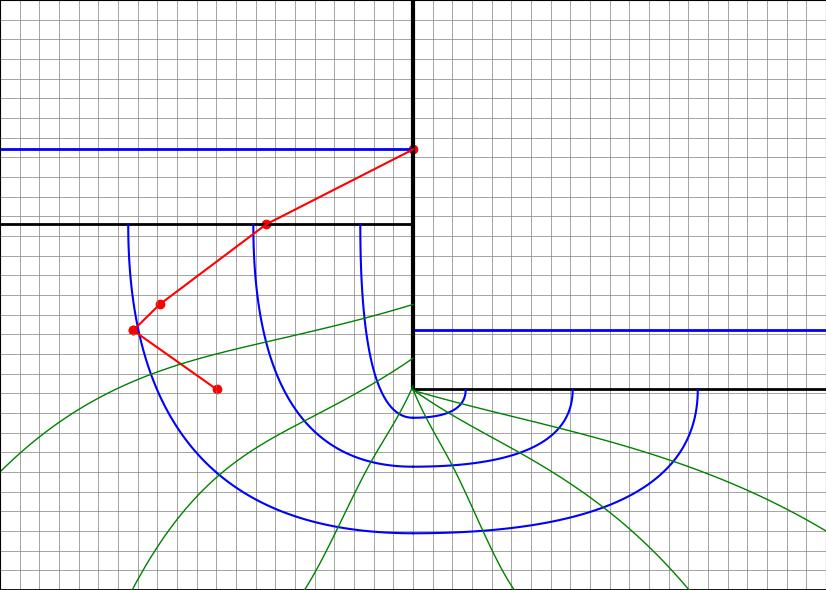
\includegraphics[width=\textwidth]{GRAFICOS/caso_1_presion_ataguia_neta.jpg}
        \caption{Caso 1 Presion Ataguia Neta}
    \end{minipage}
    \begin{minipage}{0.32\textwidth}
        \centering
        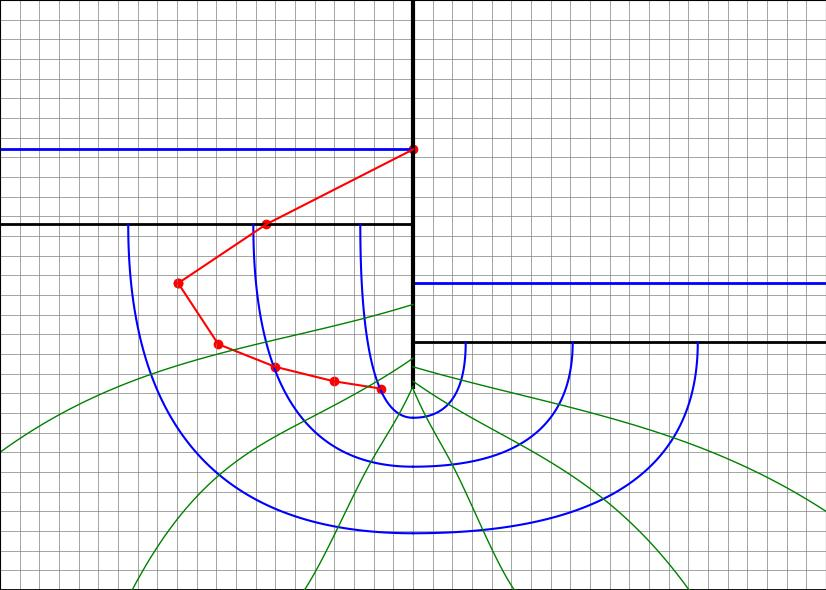
\includegraphics[width=\textwidth]{GRAFICOS/caso_2_presion_ataguia_neta.jpg}
        \caption{Caso 2 Presion Ataguia Neta}
    \end{minipage}
    \begin{minipage}{0.32\textwidth}
        \centering
        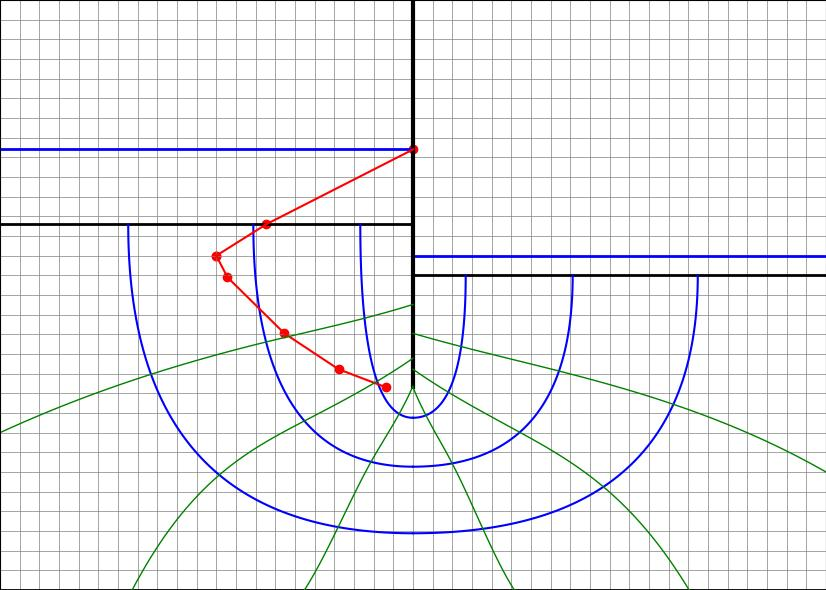
\includegraphics[width=\textwidth]{GRAFICOS/caso_3_presion_ataguia_neta.jpg}
        \caption{Caso 3 Presion Ataguia Neta}
    \end{minipage}
\end{figure}

\subsubsection{Estabilidad}

\begin{figure}[H]
    \centering
    \begin{minipage}{0.32\textwidth}
        \centering
        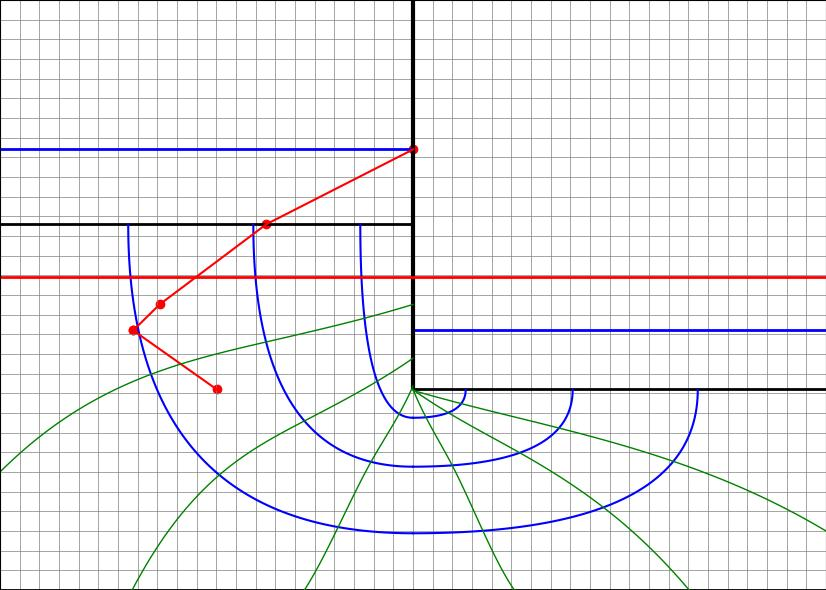
\includegraphics[width=\textwidth]{GRAFICOS/caso_1_centroide_y.jpg}
        \caption{Caso 1 Centroide}
    \end{minipage}
    \begin{minipage}{0.32\textwidth}
        \centering
        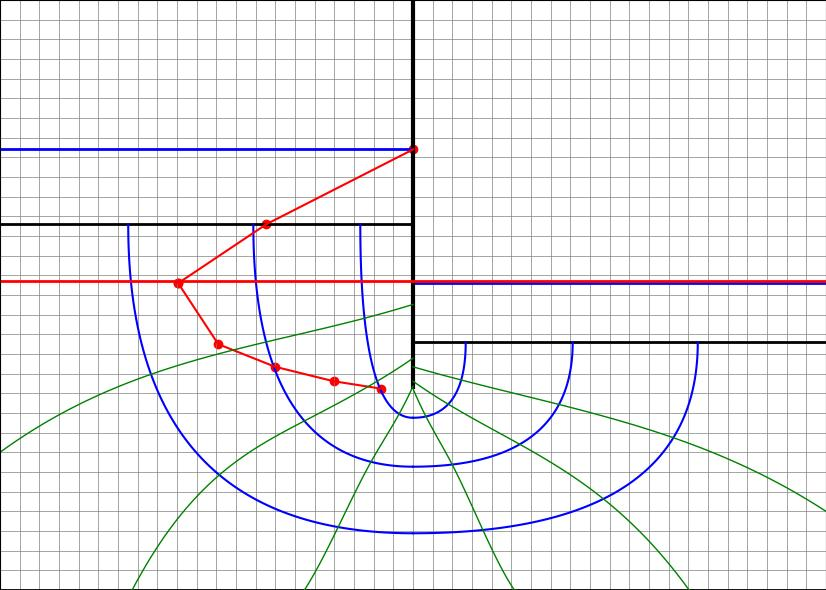
\includegraphics[width=\textwidth]{GRAFICOS/caso_2_centroide_y.jpg}
        \caption{Caso 2 Centroide}
    \end{minipage}
    \begin{minipage}{0.32\textwidth}
        \centering
        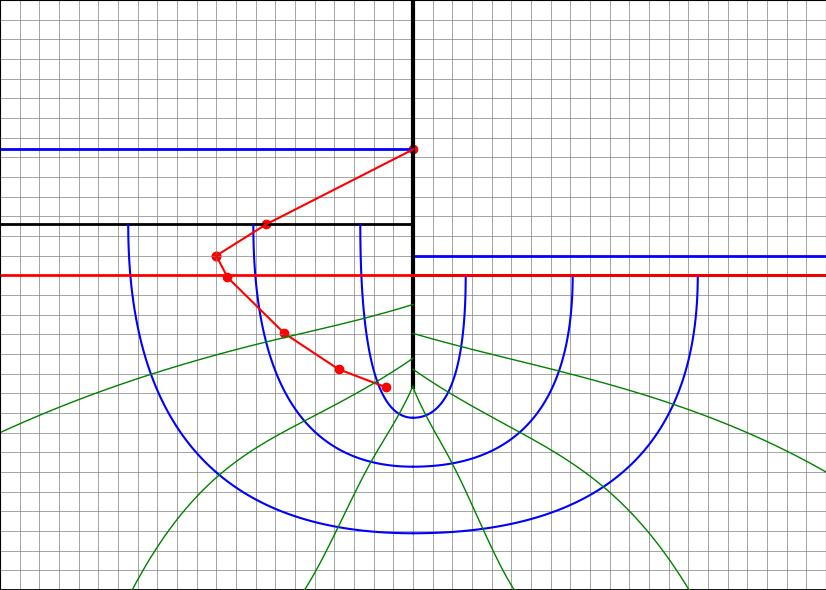
\includegraphics[width=\textwidth]{GRAFICOS/caso_3_centroide_y.jpg}
        \caption{Caso 3 Centroide}
    \end{minipage}
\end{figure}


